\documentclass[tikz,border=15pt]{standalone}
\usepackage{tikz}
\usetikzlibrary{shapes.geometric, arrows.meta, positioning, calc}

\begin{document}

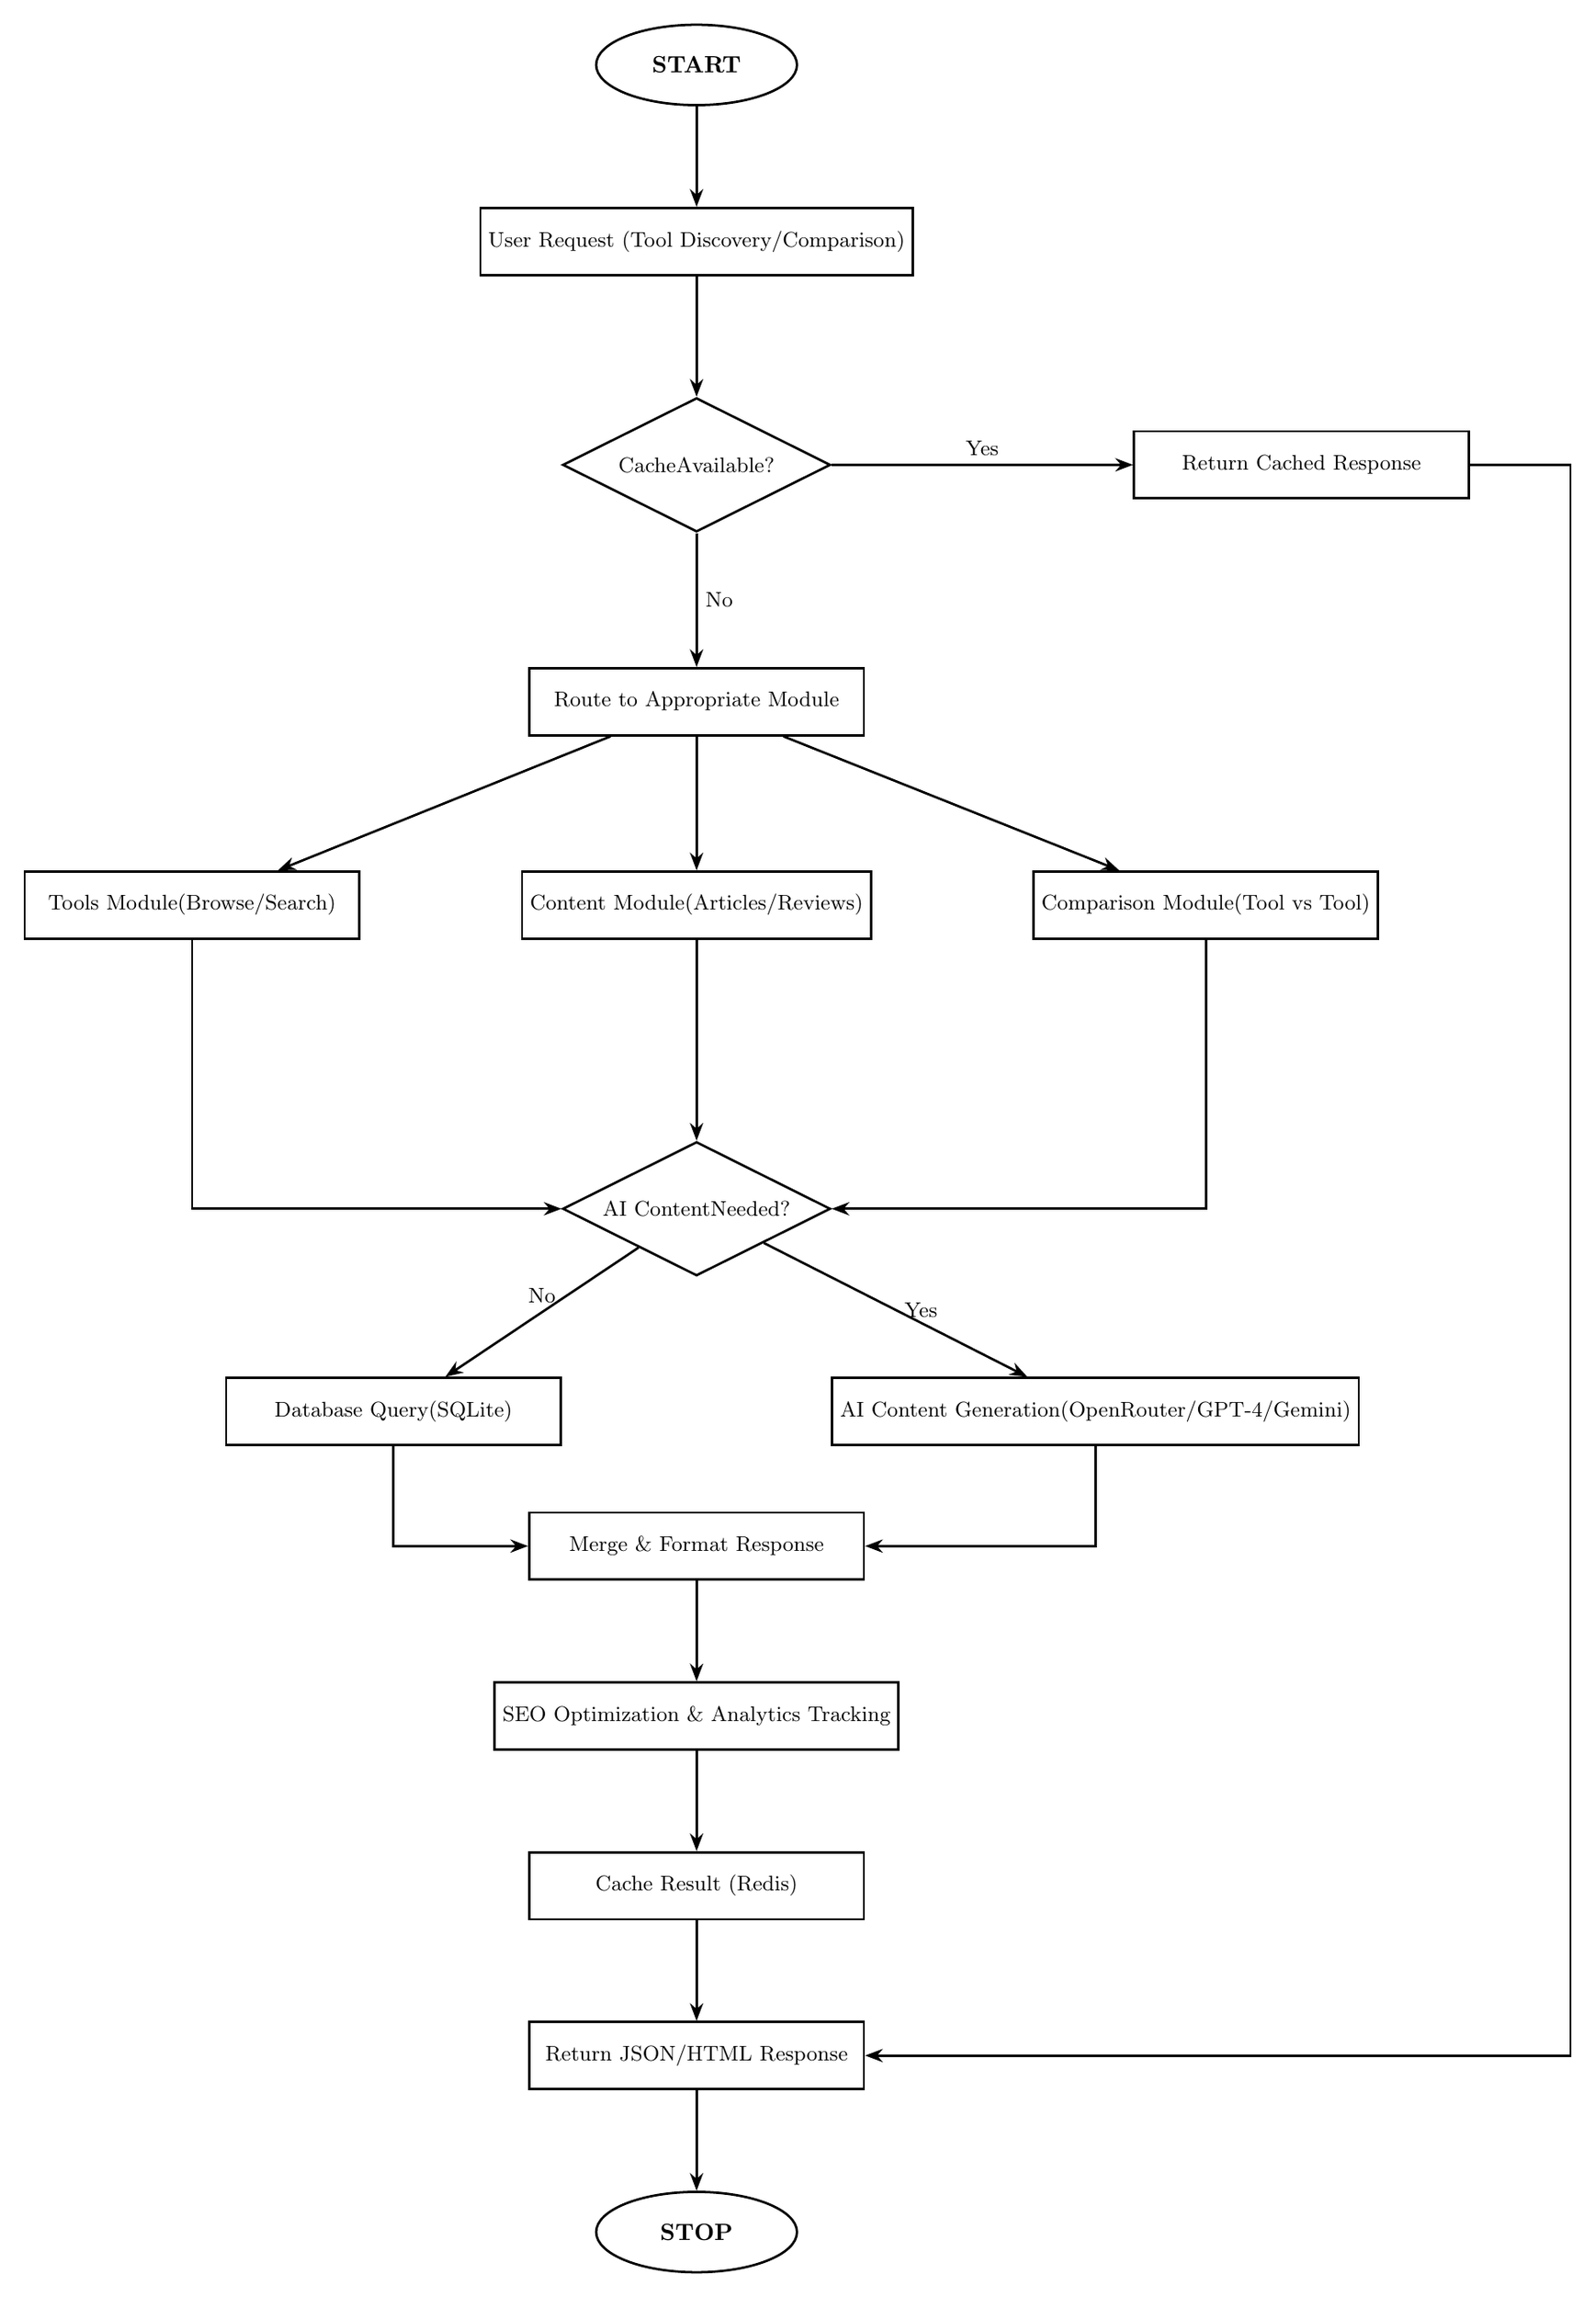
\begin{tikzpicture}[
    node distance=1.5cm,
    startstop/.style={ellipse, minimum width=3cm, minimum height=1.2cm, text centered, draw=black, line width=1pt, font=\bfseries},
    process/.style={rectangle, minimum width=5cm, minimum height=1cm, text centered, draw=black, line width=1pt, font=\small},
    decision/.style={diamond, minimum width=4cm, minimum height=2cm, text centered, draw=black, line width=1pt, aspect=2, font=\small},
    arrow/.style={->,>=Stealth,line width=1pt}
]

% Start
\node[startstop] (start) {START};

% User Request
\node[process, below=1.5cm of start] (request) {User Request (Tool Discovery/Comparison)};

% Check Cache
\node[decision, below=1.8cm of request] (cache) {Cache\\Available?};

% Cached Response
\node[process, right=4.5cm of cache] (cached) {Return Cached Response};

% Route Request
\node[process, below=2cm of cache] (route) {Route to Appropriate Module};

% Three parallel modules
\node[process, below left=2cm and 2.5cm of route] (tools) {Tools Module\\(Browse/Search)};
\node[process, below=2cm of route] (content) {Content Module\\(Articles/Reviews)};
\node[process, below right=2cm and 2.5cm of route] (comparison) {Comparison Module\\(Tool vs Tool)};

% AI Check
\node[decision, below=3cm of content] (ai-check) {AI Content\\Needed?};

% Generate AI Content
\node[process, below right=2cm and 1cm of ai-check] (ai-gen) {AI Content Generation\\(OpenRouter/GPT-4/Gemini)};

% Database Query
\node[process, below left=2cm and 1cm of ai-check] (db) {Database Query\\(SQLite)};

% Merge Results
\node[process, below=3.5cm of ai-check] (merge) {Merge \& Format Response};

% SEO & Analytics
\node[process, below=1.5cm of merge] (seo) {SEO Optimization \& Analytics Tracking};

% Cache Result
\node[process, below=1.5cm of seo] (cache-save) {Cache Result (Redis)};

% Return Response
\node[process, below=1.5cm of cache-save] (response) {Return JSON/HTML Response};

% Stop
\node[startstop, below=1.5cm of response] (stop) {STOP};

% Arrows
\draw[arrow] (start) -- (request);
\draw[arrow] (request) -- (cache);
\draw[arrow] (cache) -- node[above, font=\small] {Yes} (cached);
\draw[arrow] (cache) -- node[right, font=\small] {No} (route);

% Cached response loops back to final response
\draw[arrow] (cached.east) -- ++(1.5,0) |- (response.east);

% Route to modules
\draw[arrow] (route) -- (tools);
\draw[arrow] (route) -- (content);
\draw[arrow] (route) -- (comparison);

% Modules to AI check
\draw[arrow] (tools.south) |- (ai-check.west);
\draw[arrow] (content) -- (ai-check);
\draw[arrow] (comparison.south) |- (ai-check.east);

% AI check decision
\draw[arrow] (ai-check) -- node[right, font=\small] {Yes} (ai-gen);
\draw[arrow] (ai-check) -- node[above, font=\small] {No} (db);

% Both paths to merge
\draw[arrow] (db.south) |- (merge.west);
\draw[arrow] (ai-gen.south) |- (merge.east);

% Sequential flow
\draw[arrow] (merge) -- (seo);
\draw[arrow] (seo) -- (cache-save);
\draw[arrow] (cache-save) -- (response);
\draw[arrow] (response) -- (stop);

\end{tikzpicture}

\end{document}
